\documentclass[report]{subfiles}
\begin{document}
\section{Differential Pair}
%Doris

The Differential Pair circuit, as shown in Figure \ref{fig:Differential_pair_circuit}, is composed of two source followers with a common Fixed Current Source, $M_b$, with the bias voltage, $V_b$. The transistors, $M_1$ and $M_2$, have variable voltage inputs, $V_1$ and $V_2$, respectively, and share a common source, node V, which also acts as the drain of $M_b$. 

\begin{figure}[htbp]
  \centering
  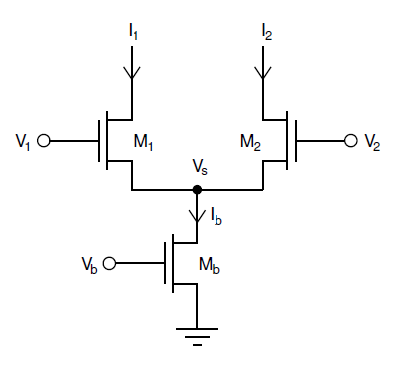
\includegraphics[scale=0.8]{pics/Differential_pair_circuit.png}
  \caption{Differential Pair Circuit}
  \label{fig:Differential_pair_circuit}
\end{figure}


The output current is proportional to the difference in the input voltages according to: 

\begin{equation}
I_1 = I_b\frac{e^{\kappa V_1}}{e^{ \kappa V_1}+e^{\kappa V_2}} = \frac{I_b}{1+ e^{\kappa(V_2-V_1)}}  \geq 0
\end{equation}
\begin{equation}
I_2 = \frac{I_b}{1+e^{\kappa(V_1-V_2)}} \geq 0
\end{equation}

Before the currents $I_1$ and $I_2$ are input, the Differential pair is off because the drain of $M_b$ (node V) is off. Once $I_1$ and $I_2$ are on and in saturation, they will charge node V to turn on $M_b$ and put $I_b$ into saturation. The transistor with the lower input voltage ($V_1$ or $V_2$) will act as a drain choke and allow less current through its drain. The losing transistor will see its source voltage (node V) increase and thus fall out of saturation. 


 \begin{figure}[htbp]
  \centering
  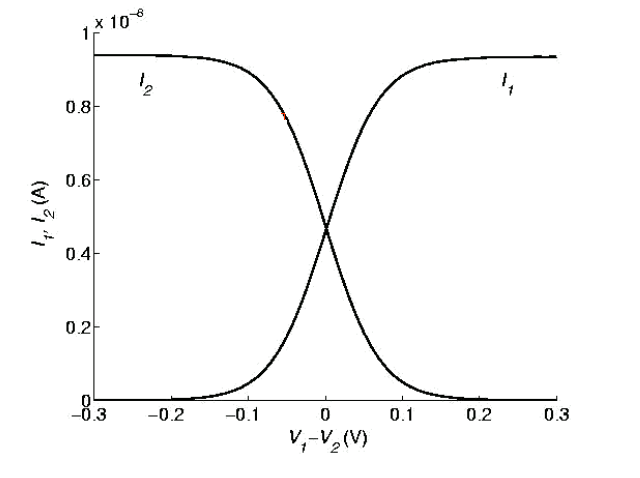
\includegraphics[scale=0.6]{pics/I-V_characteristics_of_Differential_pair.png}
  \caption{I-V characteristics of Differential pair}
  \label{fig:I-V_characteristics_of_Differential_pair}
\end{figure}




\begin{figure}[htbp]
  \centering
  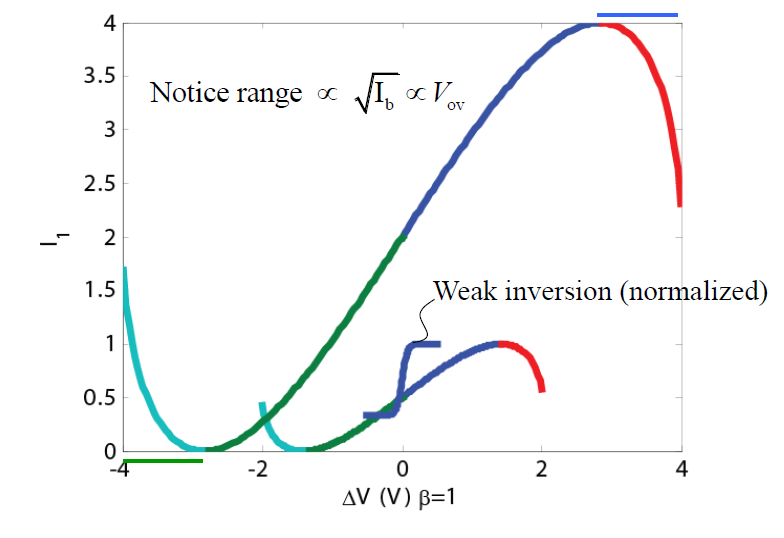
\includegraphics[scale=0.6]{pics/Differential_pair_in_weak_strong_inversion.png}
  \caption{I-V characteristics of Differential pair with reference to input voltage difference in weak $\&$ strong inversion}
  \label{fig:Differential_pair_in_weak_strong_inversion}
\end{figure}


\begin{figure}[htbp]
  \centering
  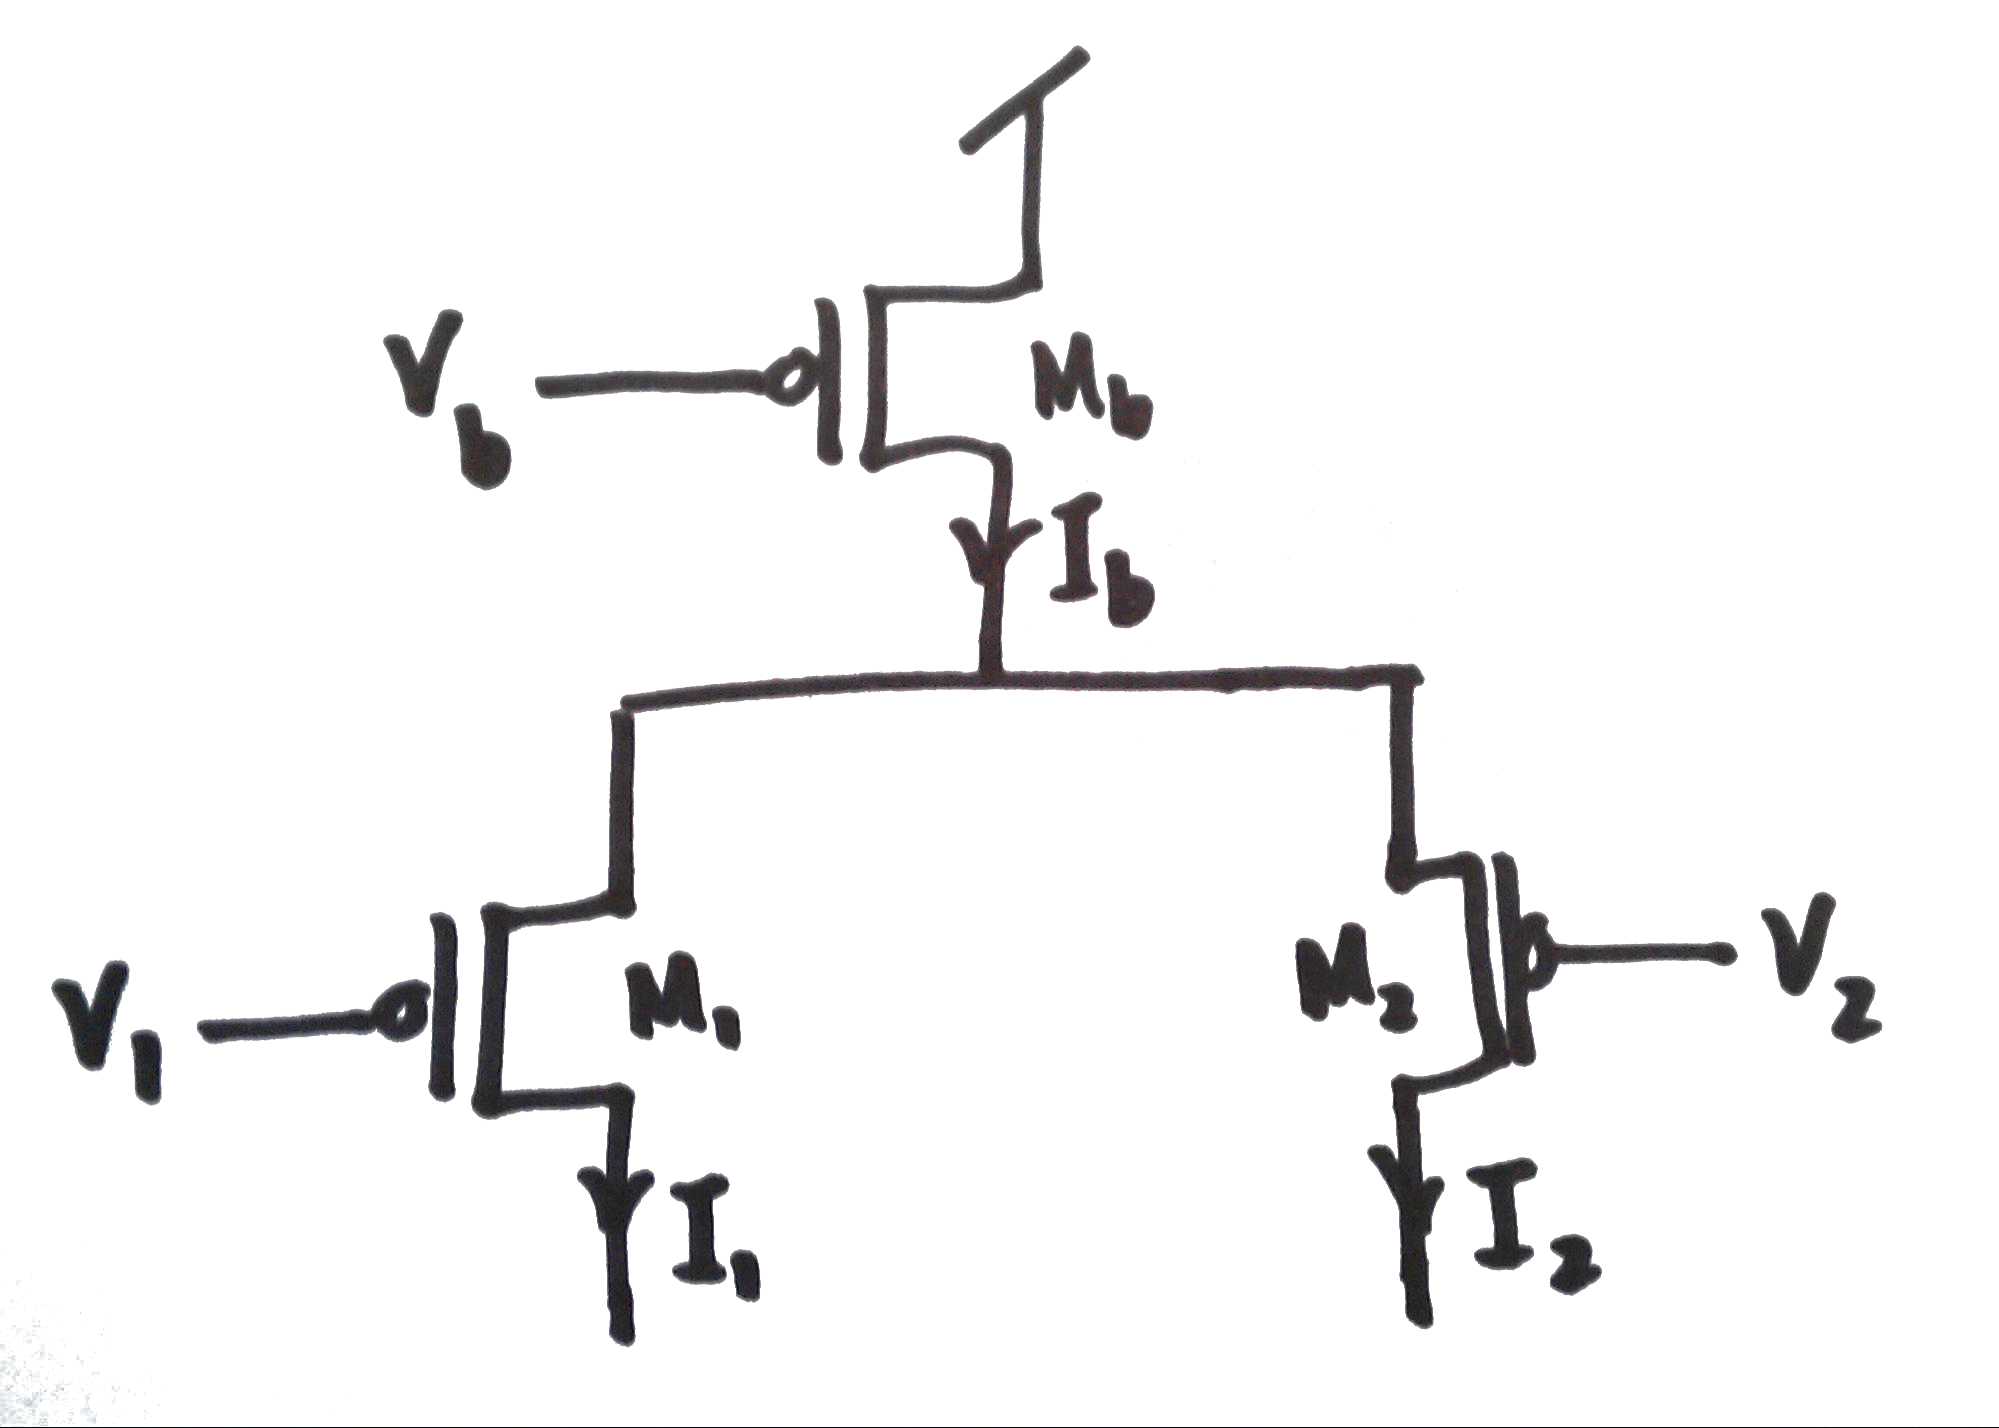
\includegraphics[scale=0.2]{pics/pFET_Differential_pair_circuit.png}
  \caption{pFET Differential pair $\rightarrow$ flipped w bias on top connected to Vdd, and M1, M2 sinking current}
  \label{fig:pFET_Differential_pair_circuit}
\end{figure}
\end{document}